%!TEX root = vmf_main.tex

\section{Application Examples}

\subsection{Music Retrieval and Prediction using Sparse Distributed Memory}

A major advantage to using VMF is that it makes applications reliant on vectors much more accessible and convenient. One such example is storage and retrieval of music a sparse distributed memory \citep*{Kane88, Roge89}. A sparse distributed memory is an associative memory model proposed by Pentti Kanerva which unlike the standard random-access memory model, allows data to be retrieved using a memory address which is suffiently close to the actual storage location rather than the exact address where the data is stored. This concept gives sparse distributed memories special properties which make them resiliant to noise, errors and queries using partially complete memory addresses. Although Kanerva's original model works with address and data vectors consisting of binary bit values, improvements were made on the original model allowing an extended sparse distributed memory which works with vectors of integers for address and data vectors \citep*{Snai13}. Since VMF is primarily composed of integer vectors, this extension to the sparse distributed memory model is extremely valuable and essential for applications involving VMF.



\subsection{Piano Roll Visualization}

One method to quickly observe the general contour and structure of a piece of music is to visualize the music in a piano roll format. This is also a valuable tool for illustrating melodic contour and rhythmic composition to those who are unfamiliar with conventional music notation (an application of this type of representation is common in music and rhythm based video games). Music stored in the Vector Music Format can be easily converted to a piano roll graphical representation due to the structure of a VMF file.

\subsubsection{Visualizing VMF}

One of the key features of the Vector Music Format is that every ``tick'' has the same temporal value. Because of this feature, it is best that the x-axis (time) uses ticks in increments of one unit. For the y-axis, as in all piano roll visualizations, a horizontal division should be used for each key on the piano keyboard. The lowest pitches are placed at the bottom of the y-axis and the highest pitches are placed at the top of the y-axis. This axis configuration allows the reader to easily view rhythmic structure by reading the visualization from left to right and to easily view melodic countour by reading the visualization in the vertical sense.

Once the two axes are properly prepared, the contents of the VMF body can be plotted by iterating through the tick vectors one by one. Within each tick vector, the same process is repeated for each of the parts or voices contained within. First the attack dimension must be evaluated: if the value is 0, then there is a silence at this tick and the next tick can be evaluated. If the value is 1, then a rectangular segment is opened at the current tick position for the pitch depicted by the pitch class and octave dimensions of the vector. Finally, if the value of the attack dimension is 2, then the note is being sustained from a previous tick and the rectangular segment which was previously opened is extended. If the last vector had a value of 2 in the attack dimension and it is followed by a vector with a value of 1, the rectangular segment is closed and a new one is opened at that position to indication a new note attack. If the last vector had a value of 2 in the attack dimension and it is followed by a vector with a value of 0, the rectangular segment is simply closed and silence (empty space) follows in the current tick. This behavior can be summarized in the extended finite state machine diagram in \ref{fig:visualizationStateMachine}. A Python implementation of this procedure is available at \href{https://github.com/project-schumann/vmf-visualization}{Github} illustrating how this visualization can be easily generated with a single traversal of a VMF file by using the ruls illustrated in the finite state machine presented in \ref{fig:visualizationStateMachine}. A piano roll visualization of the last movement of J.S. Bach's BWV 108 genedated by this script is shown in \ref{fig:bwv108PianoRoll}.

\begin{figure}
  \begin{center}
    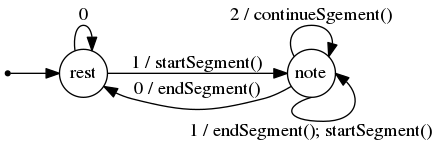
\includegraphics[scale=0.75]{resources/visualizationFSM}
    \caption{Visualization State Machine}
    \label{fig:visualizationStateMachine}
  \end{center}
\end{figure}

\begin{figure}
  \begin{center}
    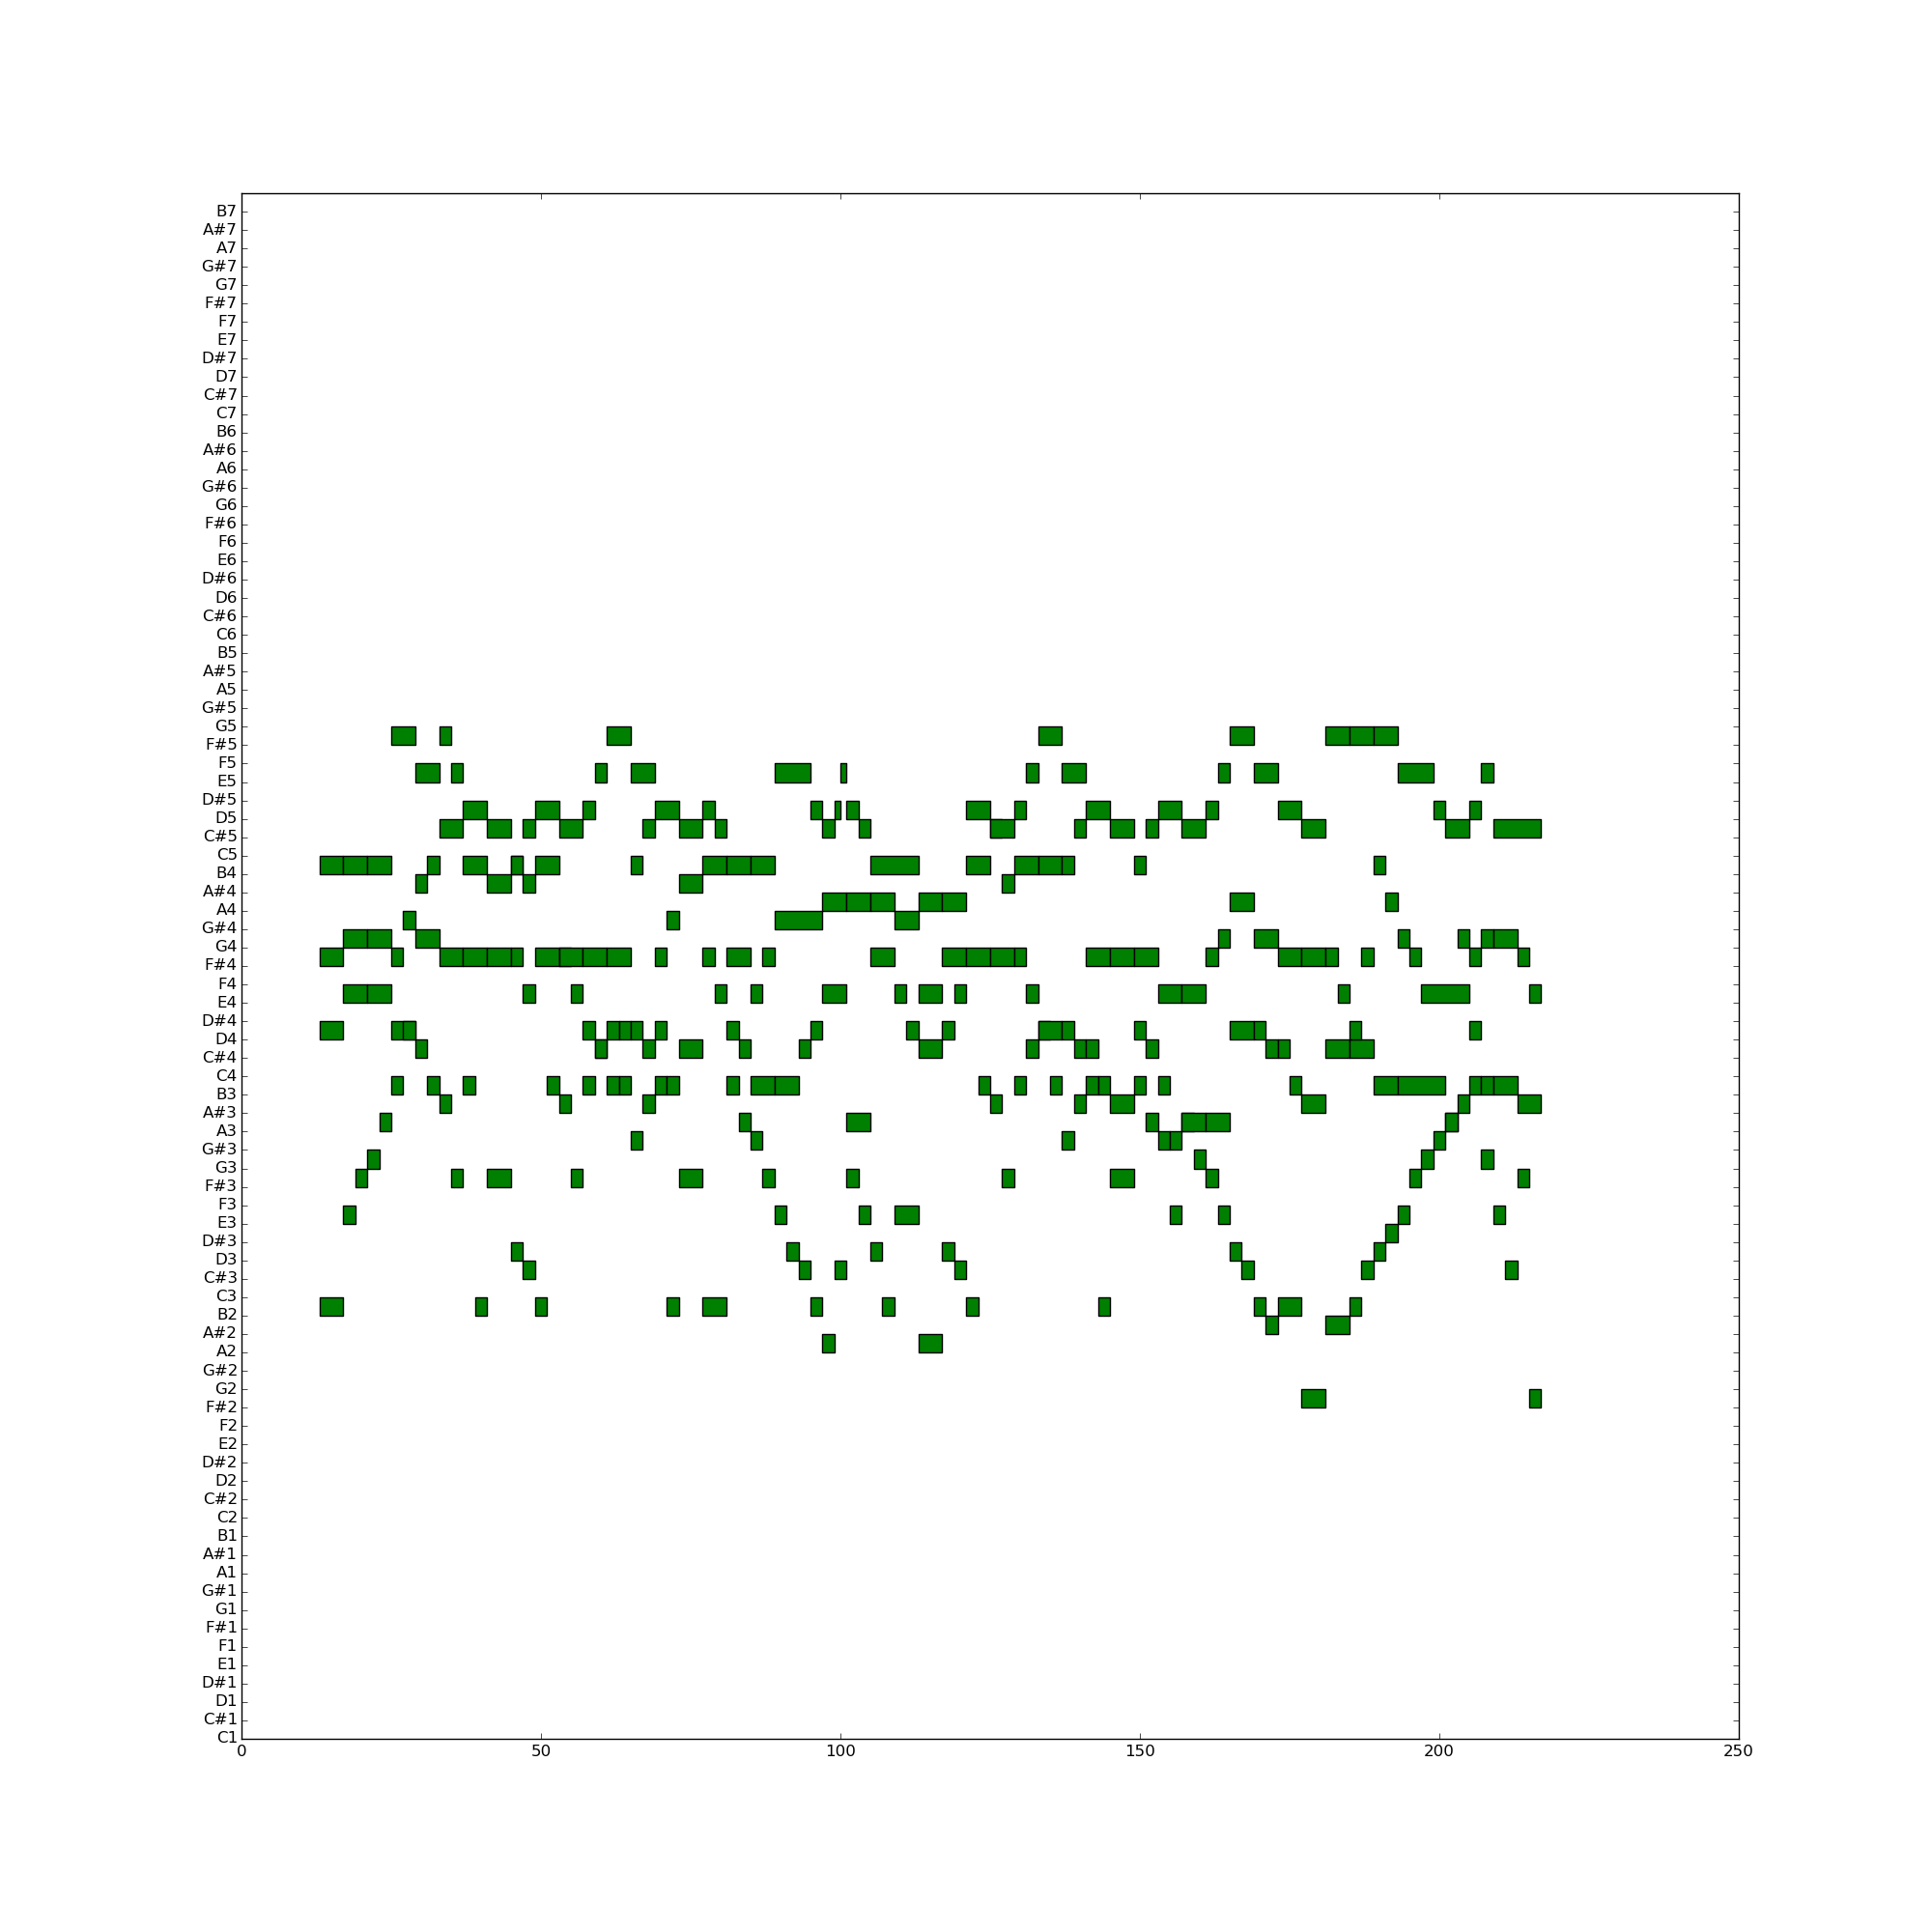
\includegraphics[scale=0.35]{resources/bwv108PianoRoll}
    \caption{Piano Roll Visualization of J.S. Bach BWV 108, Last Movement}
    \label{fig:bwv108PianoRoll}
  \end{center}
\end{figure}

\subsubsection{MIDI Visualization}

When creating a visualization directly from a MIDI file, the algorithm used depends on the type of MIDI file used. As described in ``Beyond MIDI'' \citep*{HeSe97}, there are three possible types of MIDI files; format 0, format 1, and format 2. Format 0 restricts data to a single track, format 1, allows multiple independent melodic tracks which are all synchronized to a single time line, and format 2 allows tracks which are temporally independent. When dealing with a format 0 or format 1 MIDI file, constructing the visualization is similar to visualizing a VMF file by plotting notes on the timeline by observing the note-on and note-off MIDI messages. When dealing with format 2 MIDI files, some additional work is necessary to synchronize all tracks to the same time line before plotting notes on the timeline.

\subsubsection{Humdrum Visualization}

When using a Humdrum file using the **kern format as as source for a piano roll visualization, a pre-processing step is necessary to achieve the same accuracy that VMF provides. In **kern, each pitch token is given a duration value. These duration values are equivalent to rhythmic durations seen in western music notation (ex. eighth note, sixteenth note, ...). To build the time axis of a piano roll visualization and plot notes, the largest common denominator of all the duration values to display must be determined to be used as the basic time unit. For example, if the music in \ref{fig:voicesExample} was encoded as a **kern Humdrum file, a pre-processing stage is required to determine that the eighth note is the greatest common denominator of all duration values in the piece to be visualized. Once this unit is determined, notes can be plotted by calculating how many duration units is necessary to represent each note's length accurately. In the case of the music in \ref{fig:voicesExample}, an eighth note requires one unit, a quarter note requires two units, and a half note requires four units.

By following this procedure, a **kern Humdrum file can be visualized, but the pre-processing step adds extra complexity which is not present when using a VMF file as a source.

\subsubsection{MusicXML Visualization}

Like VMF and MIDI, MusicXML encodes duration using a ``tick'' system where note durations are described in terms of subdivisions of a quarter note. In the simplest of cases, this lends itself well to piano roll visualization as in the case of VMF, however, MusicXML has some differences in this system which can cause complications when constructing a visualization of this nature. In polyphonic music, MusicXML allows different parts to use a ticks of a different value to describe note duration. For example, it is acceptable for one part to have a tick value of one third of a quarter note and another part to have a tick value of one half of a quarter note. In a case like this, it would be necessary to convert all parts to use a common tick value to facilitate visualization. Finally, MusicXML also allows the value of a tick to change in the middle of a part. Like the last case, the entire part would have to be converted to use a common tick value for the same reasons.

With any of the described formats, piano roll visualization is possible, but in some cases, varying degrees of pre-processing is necessary before the visualization can be constructed. VMF provides an advantage over these other formats as no pre-processing or computation is necessary to construct the visualization.